\documentclass[12pt,a4paper]{article}
\usepackage[margin=1in]{geometry}
\usepackage{graphicx}
\usepackage{amsmath}
\usepackage{amssymb}
\usepackage{booktabs}
\usepackage{multirow}
\usepackage{hyperref}

% Title and author information
\title{SkinCar: Pressure‐Driven Touch Robot with Localization}
\author{Qiancheng Hu, Liangyu Chen, Bingkun Huang\\Institute for Cognitive Systems, Technische Universit\"{a}t M\"{u}nchen}
\date{\today}

\begin{document}

\maketitle

\begin{abstract}
Traditional mobile robots often rely on joysticks or keyboards, creating a disconnect between the user and the machine. This project introduces \emph{SkinCar}, a four-wheeled robot that you steer by pressing touch-sensitive pads on its body. As the robot moves, its movement can be shown in simulator and a map of its surroundings is built by data collected from its sensors. The system uses a straightforward mix of computing boards and software frameworks to process touch input, control the motors, and perform mapping at the same time. 

\begin{figure}[htbp] % Use flexible placement options
    \centering
    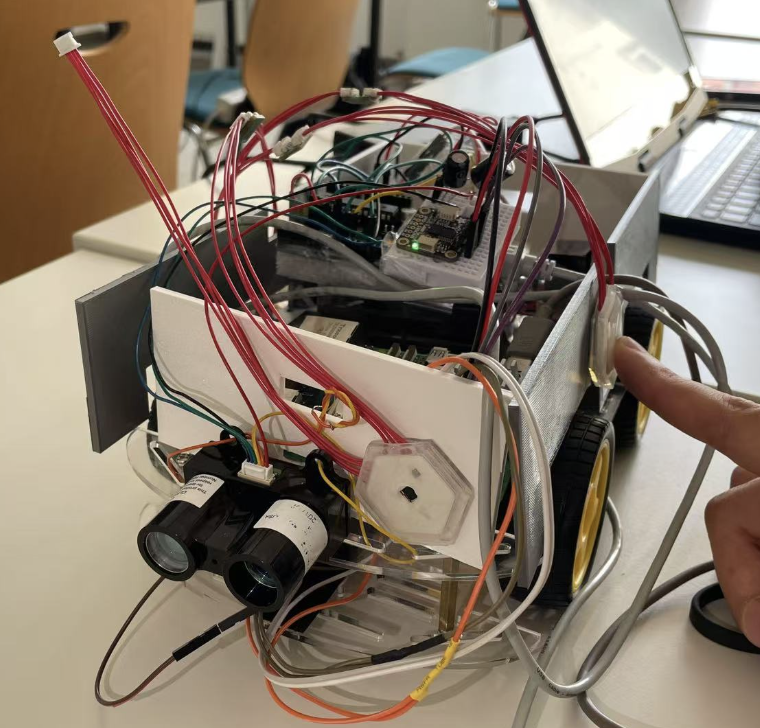
\includegraphics[width=0.5\linewidth]{car.png}
    \caption{System-level overview of SkinCar architecture}
    \label{fig:system-diagram}
\end{figure}
\section{Introduction}

People naturally move things by pushing and pulling them, but most robots are controlled with devices like joysticks or keyboards, which can feel awkward. Tactile sensors—robot “skin” that can feel pressure—let us interact with machines more directly.

Our project adds such touch-sensitive pads to the sides of a small robot. When you press a pad, the robot understands which way to move. At the same time, its sensors help it track its position and map the space around it. A simple mix of computer boards and software keeps everything running smoothly, so the robot can follow your touches while learning about its environment.

In this report, we talk about the main challenges we faced, how we connected the parts together, and what we learned from our tests.

\section{Hardware Architecture\label{sec:hardware}}

The SkinCar platform integrates mechanical components, control electronics and sensors to achieve tactile input, motion control and environmental perception.  Figure 1 illustrates the main modules and their interactions.

\subsection{Raspberry~Pi~5: System Controller}
At the core of the system lies a Raspberry~Pi~5 single‑board computer running ROS~2 Humble.  It executes high‑level algorithms including tactile interpretation, sensor fusion and SLAM.  The Pi interfaces with peripheral devices using I\textsuperscript{2}C, UART and USB serial buses and communicates with an Arduino Uno over a serial link.  A dedicated 5~V/3~A power supply ensures stable operation; additional capacitive decoupling protects against voltage fluctuations under load.  Despite its improved processing power over earlier Pi models, the Pi~5 has limited random‑access memory, necessitating careful management of memory during package compilation, as discussed later.

\subsection{Arduino Uno: Motor and Sensor Interface}
The Arduino Uno microcontroller executes low‑level tasks requiring precise timing, namely pulse‑width‑modulated (PWM) motor control and LIDAR sensor polling.  Running on an Atmega328P at 16~MHz, it provides four PWM outputs and multiple digital I/O lines.  The firmware uses a lightweight cooperative scheduler to interleave motor control with LIDAR acquisition without pre‑emptive multitasking.  Data are transmitted to the Raspberry~Pi via serial communications in a compact ASCII packet format, minimizing bandwidth demands.  Segregating time‑critical functions on the Uno reduces latency and frees the Pi to run compute‑intensive algorithms .

\subsection{Drive System and Motor Drivers}
The robot employs four brushed DC gear motors fitted with optical encoders, arranged in differential drive configuration. A single L298N dual H-bridge driver controls all four motors, with the two left motors wired in parallel to channel A and the two right motors to channel B. The driver interfaces with Arduino pins as follows: ENA (pin 5) for left-side PWM control, IN1/IN2 (pins 6-7) for left-side direction; ENB (pin 9) for right-side PWM, IN3/IN4 (pins 10-11) for right-side direction.

The motors operate at 6-9V from a dedicated battery pack, while the L298N logic circuits use the 5V rail. Establishing a common ground between the L298N, Arduino, and Raspberry Pi proved essential—without it, floating logic levels caused erratic motor behavior. The parallel motor configuration on each channel doubles the current draw, requiring adequate power supply capacity and thermal management of the L298N heat sink.

\subsection{Tactile Interface: HEX-o-SKIN Modules}
Four HEX-o-SKIN modules from TUM ICS provide tactile sensing. Each hexagonal module contains three force-sensitive cells measuring normal forces up to 10N. The modules are mounted with fixed IDs: 1 (front), 2 (left), 3 (rear), and 4 (right). They connect to the Raspberry Pi via USB using internal UART-to-USB converters at 115200 baud, drawing power directly from the USB bus. The USB interface requires the TUM ICS driver framework running in a Docker container due to its ROS1 dependencies.

\subsection{IMU and Odometry}
For orientation sensing, we employ the Hillcrest Labs BNO085 inertial measurement unit, which outputs raw inertial data including angular velocity and linear acceleration. A complementary filter processes these signals to estimate the robot’s orientation in quaternion form. Wheel encoders provide incremental counts proportional to wheel rotations, allowing computation of linear displacement. The filtered IMU orientation and encoder-derived motion are subsequently fused to obtain robust pose estimates, mitigating drift inherent to dead reckoning. Odometry messages are published at 50Hz in ROS2 format. We encountered occasional communication failures caused by connector loosening due to vibrations; these were resolved by reinforcing the solder joints to improve mechanical stability.

\subsection{LiDAR and Environmental Sensing}
A Garmin LIDAR-Lite v3 provides distance measurement from 5cm to 40m. The sensor communicates via I\textsuperscript{2}C (address 0x62) and operates at 5V, drawing up to 135mA during measurements. Direct connection to the Raspberry Pi would damage its 3.3V GPIO, so the Arduino serves as an I\textsuperscript{2}C proxy. The LiDAR connects to Arduino pins A4 (SDA) and A5 (SCL) with 4.7k$\Omega$ pull-ups to 5V. Power stability requires 220$\mu$F and 470$\mu$F capacitors in parallel (690$\mu$F total) at the sensor's power pins---insufficient capacitance causes voltage ripple and measurement errors.

\subsection{Power Supply and Stability}
The robot uses separate power rails for logic and actuation: a 5V rail supplies the Raspberry Pi, Arduino and e-skin modules, while a 9V rail drives the DC motors. Two battery packs provide 9V and 4.5V (three AAA cells) respectively; the latter is regulated to 5V via a DC--DC converter. Decoupling capacitors of 220$\mu$F and 470$\mu$F in parallel (totaling 690$\mu$F) stabilize the LIDAR's supply, addressing the voltage ripple issues we encountered with smaller capacitance values. The electronics are mounted on an acrylic chassis with compartments separating high-current and sensitive analog sections to reduce electromagnetic interference. Fuses, diodes and voltage regulators protect components against overcurrent and reverse polarity.

\subsection{Mechanical Structure}
The chassis consists of laser-cut acrylic plates housing the motors, LiDAR mount, electronics and battery holders. An acrylic deck isolates the sensor board from vibrations caused by motor motion. The four-wheeled configuration ensures stability while allowing the robot to traverse indoor environments. Overall, the hardware achieves a balance between affordability, compatibility and performance. The modular design facilitates debugging and future expansion.
\begin{figure}[htbp]
    \centering
    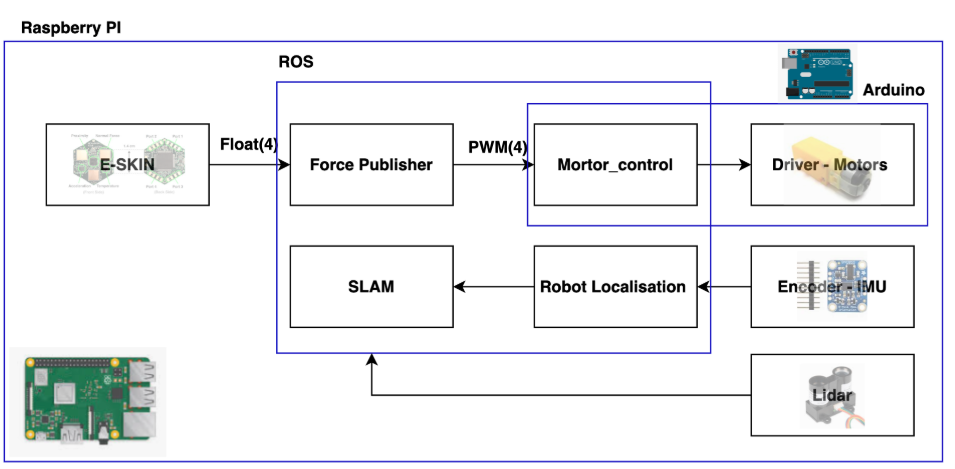
\includegraphics[width=1\linewidth]{figure1.png}
    \caption{Hardware integration overview (conceptual). The Raspberry~Pi performs high-level computation and communicates with the Arduino, e-skin, IMU and encoders. The Arduino handles PWM motor control and LIDAR sampling, relaying data to the Pi. Dual voltage rails and capacitors ensure power stability.}
    \label{fig:enter-label}
\end{figure}

\section{Methodology\label{sec:methodology}}

The software stack couples legacy drivers with modern navigation libraries through a hybrid ROS~1–ROS~2 architecture.  Figure\,\ref{fig:software} summarizes the primary nodes, topics and data flows.  We describe the execution flow from boot to operation, detail ROS~1 and ROS~2 nodes, explain the bridge configuration and highlight the Arduino firmware design.  We also discuss the practical challenges encountered during software development, including cross‑platform communication, memory constraints and package compilation on a nascent Raspberry~Pi platform.

\subsection{System Boot and Operation Flow}
Upon powering the robot, the Raspberry~Pi boots and initializes ROS~2 nodes. A ROS~1 Docker container is then launched to host the TUM ICS e-skin drivers. Sensors are initialized, and the sensor data are calibrated and fused, and the ros\_bridge is started to link topics between ROS versions. Finally, tactile control is activated. During operation, tactile inputs from the HEX-o-SKIN modules are processed by the force\_publisher\_node, which publishes averaged force values to \texttt{/skin\_forces} at 30Hz. The motor\_control.py script subscribes to these force messages, determines the direction with maximum force, maps the force magnitude to PWM values (80-255), and sends motor commands directly to the Arduino via serial (\texttt{/dev/ttyACM0}) in the format \texttt{pwmA,dirA,pwmB,dirB}. Simultaneously, the lidar\_publisher node receives distance measurements from the Arduino via the same serial port and publishes them as \texttt{sensor\_msgs/LaserScan} on \texttt{/scan} for ROS~2 consumption via the bridge. Odometry messages are generated from encoder and IMU readings in the native ROS~2 environment. We employ the robot\_localization and slam\_toolbox nodes to fuse these data streams and build occupancy maps of the environment. Finally, the robot's movement and the generated map can be visualized in a simulator running on a laptop.

\subsection{ROS~1 Nodes in Docker}
The TUM ICS e-skin drivers require ROS~1, so we use their Docker container with ROS~Noetic. This container runs two packages: skin\_force\_publisher for tactile control and lidar\_publisher for distance measurement relay.

\subsubsection{skin\_force\_publisher Package}
This package contains two nodes working in sequence. The force publisher node initializes by loading the patch configuration from default.xml, which defines four e-skin units with IDs 1-4 corresponding to front, left, rear, and right positions. It establishes data connections through the TfMarkerDataPatch interface and enters a 30Hz polling loop. In each cycle, the node calls dataFromId() for each unit, retrieves the three-element force vector, computes the average, and publishes the four averaged values as a Float64MultiArray on /skin\_forces.

The motor control node subscribes to /skin\_forces and processes each incoming message by first identifying the maximum force among the four sensors. If this maximum exceeds the 0.003 threshold, it maps the force magnitude to a PWM value using linear interpolation between 80 (minimum motor speed) and 255 (maximum). The control logic then generates motor commands based on which sensor has the maximum force: front sensor triggers backward motion (both motors reverse), rear sensor forward motion, left sensor rightward rotation, and right sensor leftward rotation. These decisions are formatted as "pwmA,dirA,pwmB,dirB" strings and transmitted via serial at 9600 baud.

The Qt dependency from the skin API requires special handling—the QT environment variable must be set to "offscreen" to prevent display initialization attempts. The launch sequence uses bash delays to ensure the skin driver completes USB enumeration before dependent nodes start.

\subsubsection{lidar\_publisher Package}
This Python node creates a serial connection to /dev/ttyACM0 and continuously reads incoming data. When it detects the "L:" prefix, it parses the subsequent digits as centimeters, validates the range (1-800cm), and applies a 10cm offset correction determined during calibration. 

The conversion to LaserScan format addresses a fundamental incompatibility: SLAM algorithms expect arrays of measurements across angular sweeps, but the LIDAR-Lite provides single-point readings. The node constructs a LaserScan message with angle\_min and angle\_max both set to zero, indicating no angular coverage. The single distance value (converted to meters) populates the ranges array, while the original centimeter reading is stored in intensities for debugging. This approach allows slam\_toolbox to interpret each message as a degenerate scan containing one valid measurement at zero degrees.

The node publishes at 20Hz to /scan, with built-in error handling for serial exceptions and invalid data formats. Range validation prevents erroneous readings from corrupting the map.

\subsubsection{Serial Resource Conflict}
Both motor\_control.py and lidar\_publisher\_node.py specify /dev/ttyACM0 as their serial port. The system functions because the Arduino firmware alternates between Serial.available() checks (receiving motor commands) and Serial.print() calls (sending distance data) in its main loop, creating unintentional time-division multiplexing. While no communication errors occurred during testing, this configuration is fragile—changes to timing or message frequency could cause data corruption. The issue remained unresolved due to time constraints and the absence of immediate failures.

\subsection{ROS~2 Nodes and Processing Pipeline}
The Raspberry Pi5 supports ROS2 exclusively through source-based installation on the host system. Since Docker containers cannot directly access the Pi's GPIO pins, hardware requiring such access—including the IMU and wheel encoders—must operate within the native ROS 2 environment. Accordingly, data acquisition from these sensors, as well as sensor fusion and mapping using \texttt{robot\_localization} and \texttt{slam\_toolbox}, are implemented entirely within the ROS2 workspace on the host.
\begin{itemize}
     \item \textbf{encoder\_node}. This node reads wheel encoder pulses from two GPIO pins on the robot’s front wheels. It calculates the left and right wheel displacements, estimates the robot’s 2D pose and velocity, and publishes \texttt{/nav\_msgs/Odometry} messages on the \texttt{/wheel\_odom} topic. It also optionally broadcasts TF transforms between odom and base\_link. 
    \item \textbf{imu\_node}. This node interfaces with the IMU, reading four types of sensor data: linear acceleration, angular velocity, magnetic field, and quaternion orientation. These values are published at 20 Hz to the \texttt{/imu/data\_raw} topic. This topic is used in a complementary filter node which subscribes to \texttt{/imu/data\_raw}, performs calibration between accelerometer and gyroscope data using an adaptive complementary filter, and publishes a calibrated IMU message to \texttt{/imu}. 
    

\begin{figure}[htbp]
    \centering
    \begin{minipage}[t]{0.45\linewidth}
        \centering
        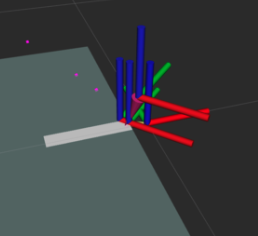
\includegraphics[width=0.9\linewidth]{image3.png}
        \caption{Odometry Estimator}
        \label{fig:left-image}
    \end{minipage}
    \hfill
    \begin{minipage}[t]{0.45\linewidth}
        \centering
        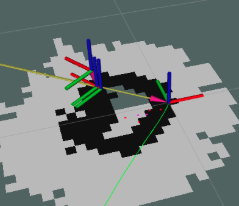
\includegraphics[width=0.9\linewidth]{image.png}
        \caption{SLAM Module}
        \label{fig:right-image}
    \end{minipage}
\end{figure}
    \item \textbf{robot\_localization}. We use the robot\_localization package to perform sensor fusion using an Extended Kalman Filter (EKF). It subscribes to topic (/imu) from the complementary filter node and (/wheel\_odom) from the encoder node. In the fusion configuration, the 2D planar position (x, y) is mainly trusted by encoder odometry, providing accurate translational motion. For yaw orientation, both encoder and IMU angular velocity data are fused together, resulting in a more stable and robust heading estimate (As shown in Figure 3).  It also continuously publishes the transform between the odom and base\_link frames.
    \item \textbf{static\_transform\_publisher}. To ensure all sensor data are correctly registered in a common coordinate frame, several static\_transform\_publisher nodes are used to define fixed transforms between each sensor and the robot's base frame. Specifically, static transforms are published from the laser\_link and imu\_link frames to base\_link. These transforms are essential for constructing a consistent and accurate TF tree, which is a prerequisite for SLAM. 
    \item \textbf{slam\_toolbox}. We use the slam\_toolbox package to perform 2D SLAM. It subscribes to the laser scan data from /scan and the fused odometry from /odometry/filtered. Using these inputs, the node builds a consistent occupancy grid map of the environment (As shown in Figure 4). It also continuously publishes the transform between the map and odom frames. The generated map is published on the /map topic as a nav\_msgs/OccupancyGrid message. 
\end{itemize}

\subsection{Communication}
The system is built on two layers of communication: internal communication between ROS1 and ROS2 on the Raspberry Pi via the \texttt{ros\_bridge}, and external communication between the Raspberry Pi and the host PC over the local network using native ROS2 DDS transport. The overall communication architecture is shown in Figure5.
\begin{itemize}
     \item \textbf{ROS~1–ROS~2 Bridge}. The \texttt{ros\_bridge} facilitates communication between the ROS 1 container (running on the Raspberry Pi) and the native ROS 2 environment. This configuration is necessary because the LiDAR sensor is interfaced via drivers inside a ROS 1 Docker container, while the rest of the system (e.g., localization, mapping) runs on the ROS~2 layer, allowing the system to access sensor data from the containerized topics.
     \item \textbf{Host-Device Communication}. The Raspberry Pi and the host PC communicate over the same local network using native ROS2 DDS-based transport. To enable seamless discovery and message exchange across machines, both devices are configured with identical environment variables (ROS\_DOMAIN\_ID). This setup allows ROS~2 nodes running on different hardware platforms to participate in a shared computational graph, facilitating tasks such as remote visualization in RViz and SLAM processing on the more powerful PC while sensor data are collected on the Raspberry Pi.


\end{itemize}

\subsection{Arduino Firmware}
The Arduino UNO firmware provides low-level hardware interface for motor control and distance sensing. The firmware is structured into three modules using PlatformIO:
\begin{enumerate}
    \item \textbf{Motor Control Module} (\texttt{motor\_control.cpp}). This module implements the \texttt{setMotor()} function that receives four parameters: PWM values (0-255) and direction bits (0/1) for each motor. It directly controls six digital pins connected to the L298N driver (Motor A: ENA=5, IN1=6, IN2=7; Motor B: ENB=9, IN3=10, IN4=11). When PWM is zero, the module explicitly stops the motor by setting all control pins low to prevent floating states.
    \item \textbf{LiDAR Interface Module} (\texttt{lidar\_sensor.cpp}). This module wraps the Garmin LIDAR-Lite library v3.0.5, which handles the I\textsuperscript{2}C communication protocol internally. The \texttt{setupLidar()} function initializes the sensor with default configuration and 400kHz I\textsuperscript{2}C speed, while \texttt{getDistance()} returns the measured range in centimeters using the library's built-in bias correction.
\end{enumerate}
The main loop (\texttt{main.cpp}) implements a simple event-driven architecture: it checks for incoming serial commands using \texttt{Serial.available()} and parses them with \texttt{sscanf()} for motor control, while a timer based on \texttt{millis()} triggers LiDAR readings every 100ms. The LiDAR data is formatted as \texttt{L:xxx} and sent via serial at 9600 baud. The Wire library provides I\textsuperscript{2}C primitives required by the Garmin library, which abstracts the complex LIDAR-Lite register operations and measurement timing. This modular structure simplifies debugging and allows independent testing of each subsystem.

\subsection{Software Development Challenges}
Several practical challenges arose during software development:
\begin{enumerate}
    \item \textbf{Cross-Platform ROS Versions}. The TUM ICS e-skin drivers were available only for ROS~1~Noetic, whereas modern navigation frameworks (e.g., slam\_toolbox and sensor fusion packages) target ROS~2. Bridging these versions required careful configuration of message conversions and topic namespaces. We created interface wrappers to minimize coupling and used dockerization to isolate the ROS~1 environment.
    \item \textbf{Hardware Access in Containers}. Running ROS~1 inside a Docker container complicated access to hardware devices. While the container could access USB devices (e-skin) and serial ports, it could not control the Raspberry~Pi's GPIO pins. Therefore, all GPIO-dependent functions (IMU and wheel encoders) remained in ROS~2 nodes running on the host. We granted the container privileges to access \texttt{/dev/ttyUSB0} and \texttt{/dev/ttyACM0} for serial communication with the Arduino.
    \item \textbf{Missing Dependencies in ROS~2 Packages}. The slam\_toolbox package failed to build due to a missing \texttt{Pose2D.msg} definition in the geometry\_msgs package. We manually copied the message file from the ROS~2 installation directory and modified the package's \texttt{CMakeLists.txt} to include it. Memory constraints on the Pi~5 required expanding swap space to 2GB using \texttt{dphys-swapfile} and restricting compilation to single-threaded mode with \texttt{MAKEFLAGS="-j1"} and \texttt{-{}-parallel-workers 1}.
    \item \textbf{Interfacing Multiple Scripts}. For the Arduino we wrote multiple firmware modules in C/C++. The default Arduino IDE struggles with multi-file projects and external libraries. Switching to PlatformIO, which uses a Makefile-like configuration, allowed us to include third-party libraries (e.g., Garmin's LIDAR-Lite library) and to compile multiple source files seamlessly.
    \item \textbf{Wireless Networking}. Development occurred over remote SSH sessions. Public Wi-Fi networks blocked local routing, and smartphone hotspots exhibited intermittent drops due to high data consumption. These instabilities often caused connection loss during code uploads or debugging. To mitigate, we configured the Pi as a Wi-Fi access point and connected our laptops directly. We also used wired Ethernet when possible to ensure reliable connectivity.
    \item \textbf{Mechanical and Electrical Reliability}. Loose physical connections frequently caused inconsistent behaviour. The IMU's connector detached due to vibrations, which we fixed by reinforcing solder joints. Without a common ground between the L298N boards, UNO and Pi, logic levels floated causing motors to spin spontaneously. Ensuring a shared ground resolved the issue. Additionally, the e-skin module's Qt-based driver attempted to create graphical windows even in headless operation, causing initialization failures. Launching with the \texttt{-{}-force-offscreen} flag resolved this issue.
\end{enumerate}
\begin{figure}[htbp]
    \centering
    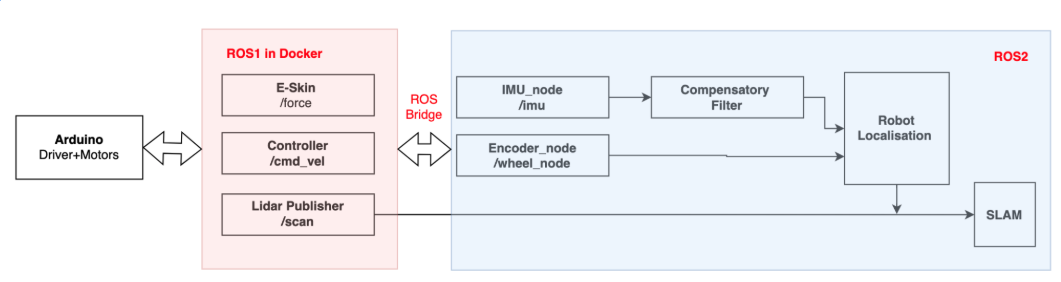
\includegraphics[width=1\linewidth]{figure2.png}
    \caption{Software architecture overview (conceptual). The Raspberry~Pi runs ROS~2 nodes for odometry, sensor fusion and SLAM. A ROS~1 Docker container hosts e-skin processing and motor control. The ros\_bridge relays sensor data between the two system. The Arduino executes firmware tasks for motor control and LIDAR polling, communicating with the Pi over serial.}
    \label{fig:enter-label}
\end{figure}

\section{Implementation Status and Development Plans}
\label{sec:experiments}

At this stage, the SkinCar platform has been built and several core features are functional, although formal experiments and user studies have not yet been conducted. The focus has been on implementing and testing individual components to ensure that the overall system operates reliably. This section summarizes what has been accomplished so far, outlines opportunities for further development, and sets out general guidelines for contributors.
\subsection{Completed Work}
The implementation achieved the following:
\begin{itemize}
\item Integrated four HEX-o-skin modules with force averaging, achieving 30Hz tactile feedback
\item Established proportional control mapping from touch intensity to motor PWM signals
\item Implemented Arduino-based hardware abstraction for motor control and LiDAR communication
\item Configured IMU and wheel encoder fusion for odometry estimation
\item Adapted slam\_toolbox to process single-point distance measurements
\item Created ROS1-ROS2 bridge for cross-version data exchange
\end{itemize}

\subsection{Limitations}
The current system has several constraints. The single-point LiDAR cannot generate complete environmental scans without mechanical rotation. The robot lacks autonomous navigation capabilities and requires continuous manual control. The mixed ROS1/ROS2 architecture increases system complexity and memory usage. The current four e-skin units provide only basic directional control without fine-grained position sensing. Open-loop motor control limits trajectory accuracy, particularly during turns.

\section{Conclusions and Future Work}
\label{sec:conclusion}

This project demonstrated that tactile sensors can provide an intuitive interface for mobile robot control. The successful integration of e-skin technology with SLAM capabilities validates the feasibility of touch-based robot navigation. The modular architecture, while complex, effectively separated hardware control from high-level processing.

Future development should focus on enhancing both sensing and autonomy capabilities. A servo-controlled scanning platform for the LiDAR would enable full 360-degree mapping during movement. Expanding the e-skin array to cover more surface area, potentially using Ethernet or PCIe for higher bandwidth, would allow precise touch localization through the skin patch reconstruction API. The recorded trajectory data could enable autonomous return-to-origin functionality, while the SLAM system could be extended with obstacle avoidance algorithms. These improvements would transform the current teleoperated platform into a semi-autonomous robot capable of safe navigation in cluttered environments.

\section{Individual Contributions}
\label{sec:contributions}

Qiancheng Hu developed the ROS nodes for e-skin force processing and LiDAR data acquisition. He integrated the Arduino firmware modules using PlatformIO and collaborated on resolving the slam\_toolbox compilation issues that arose during the ROS2 setup.

Bingkun Huang implemented the motor control software that interfaces with the L298N drivers, translating force inputs into motor commands. He performed the electrical system wiring and troubleshooting, ensuring reliable connections between all components. Additionally, he designed and 3D-printed the robot chassis and various component mounts.

Liangyu Chen configured the localization and SLAM modules, including IMU calibration and the sensor fusion pipeline using the robot\_localization and slam\_toolbox package. He established the Docker environment for ROS1 compatibility and set up the ROS bridge architecture to enable cross-version communication. Throughout the project, he maintained the Raspberry Pi development environment and resolved various dependency issues.

\section*{Acknowledgements}
We thank the Institute for Cognitive Systems at the Technical University of Munich for providing resources and support. We also thank Dr. Florian Bergner for his guidance throughout this project.

\begin{thebibliography}{99}

\bibitem{arduino}
Arduino, \textit{Arduino UNO Reference Manual}, [Online]. Available in: \texttt{Arduino\_UNO.pdf}

\bibitem{dcgear}
DC Motor Base, \textit{DC Gear Car Base Specifications}, [Online]. Available in: \texttt{DC\_Gear\_Car\_Base.pdf}

\bibitem{eskin_hw}
StretchSense, \textit{E-SKIN HEX-o-SKIN Hardware Overview}, [Online]. Available in: \texttt{E-SKIN\_\_HEX-o-SKIN\_hardware.pdf}

\bibitem{eskin_paper}
StretchSense, \textit{E-SKIN HEX-o-SKIN Technical Paper}, [Online]. Available in: \texttt{E-SKIN\_\_HEX-o-SKIN\_paper.pdf}

\bibitem{lidar}
Garmin, \textit{LIDAR-Lite v3 Operation Manual}, [Online]. Available in: \texttt{Garmin\_LIDAR\_Lite\_v3.pdf}

\bibitem{imu}
Hillcrest Labs, \textit{BNO085 IMU Datasheet}, [Online]. Available in: \texttt{IMU-bno085.pdf}

\bibitem{l298n}
STMicroelectronics, \textit{L298N Dual H-Bridge Motor Driver Datasheet}, [Online]. Available in: \texttt{L298N\_Motor\_Driver.pdf}

\bibitem{piimu}
User Guide, \textit{Raspberry Pi + IMU Integration Guide}, [Online]. Available in: \texttt{PI\_IMU\_Guide\_GPT.pdf}

\bibitem{github}
Qiancheng Hu, \textit{HSA Project Hardware Documentation}, GitHub repository,\\
\url{https://github.com/HUQiancheng/HSA_Project/tree/main/docs/hardware}

\end{thebibliography}


\end{document}